%%---------------Homework Template------------------%%
%----------------------------------------------------%
\documentclass[a4paper,11pt]{article}

%---------------code settings------------------------%
\usepackage{listings}
\usepackage{xcolor}
\definecolor{mygreen}{rgb}{0,0.6,0}
\definecolor{mygray}{rgb}{0.5,0.5,0.5}
\definecolor{mymauve}{rgb}{0.58,0,0.82}

\lstset{ %
  backgroundcolor=\color{white},   % choose the background color; you must add \usepackage{color} or \usepackage{xcolor}
  basicstyle=\footnotesize,        % the size of the fonts that are used for the code
  breakatwhitespace=false,         % sets if automatic breaks should only happen at whitespace
  breaklines=true,                 % sets automatic line breaking
  captionpos=bl,                    % sets the caption-position to bottom
  commentstyle=\color{mygreen},    % comment style
  deletekeywords={...},            % if you want to delete keywords from the given language
  escapeinside={\%*}{*)},          % if you want to add LaTeX within your code
  extendedchars=true,              % lets you use non-ASCII characters; for 8-bits encodings only, does not work with UTF-8
  frame=single,                    % adds a frame around the code
  keepspaces=true,                 % keeps spaces in text, useful for keeping indentation of code (possibly needs columns=flexible)
  keywordstyle=\color{blue},       % keyword style
  %language=Python,                 % the language of the code
  morekeywords={*,...},            % if you want to add more keywords to the set
  numbers=left,                    % where to put the line-numbers; possible values are (none, left, right)
  numbersep=5pt,                   % how far the line-numbers are from the code
  numberstyle=\tiny\color{mygray}, % the style that is used for the line-numbers
  rulecolor=\color{black},         % if not set, the frame-color may be changed on line-breaks within not-black text (e.g. comments (green here))
  showspaces=false,                % show spaces everywhere adding particular underscores; it overrides 'showstringspaces'
  showstringspaces=false,          % underline spaces within strings only
  showtabs=false,                  % show tabs within strings adding particular underscores
  stepnumber=1,                    % the step between two line-numbers. If it's 1, each line will be numbered
  stringstyle=\color{orange},     % string literal style
  tabsize=2,                       % sets default tabsize to 2 spaces
  %title=myPython.py                   % show the filename of files included with \lstinputlisting; also try caption instead of title
}

%---------------------other package--------------&
\usepackage[T1]{fontenc}
\usepackage[utf8x]{inputenc}
\usepackage[english]{babel}
\usepackage{float}
\usepackage[colorlinks=true, allcolors=blue]{hyperref}
\usepackage[parfill]{parskip}
\usepackage[a4paper,top=2cm,bottom=3cm,left=1.5cm,right=1.5cm,marginparwidth=2cm]{geometry}
\usepackage{graphicx}
\usepackage{fancyhdr}
\usepackage{titlesec}
\usepackage{amsmath}
\usepackage{amssymb}
\usepackage{indentfirst}
\setlength{\headheight}{41pt}
\setlength{\parindent}{2em}


\begin{document}

%--------------fancyhead------------%
\pagestyle{fancy}
\fancyhead[R]{Classical Electrondynamics}
\fancyhead[L]{
\includegraphics[width=4.5cm]{logo/row.png}}
\fancyfoot[R]{
\includegraphics[width=3cm]{logo/spst.png}}
%---------------title---------------%
\title{\textbf{\Huge{Homework-2}}}

%--------------author---------------%
\author{\textit{Xinzhi Li} \\\quad\\Student ID:~~$\boldsymbol{2022211084}$\\\quad\\ \textit{School of Physics Science and Technology, ShanghaiTech University, Shanghai 201210, China}\\\quad \\ \textit{Email address}:\quad lixzh2022@shanghaitech.edu.cn}


%---------------Logo----------------%
\begin{figure*}[t]
\centering

\includegraphics[width=1\columnwidth]{logo/row.png}
\end{figure*}

%--------------maketitle--------------&
\maketitle\thispagestyle{empty}
%--------------main body--------------&
\newpage
\setcounter{page}{1}

\begin{enumerate}
  \item Point charge in the presence of a charged conducting sphere. A point charge $q$ is at $(0,0,d)$. A conductor sphere with total charge $Q$ and with radius $a$ is placed at the origin. $Q$ and $q$ have the same sign, and $d>a$. Please answer the following questions:
  \begin{enumerate}
    \item Calculate the electric potential distribution outside the sphere using method of images.
    \begin{figure}[h]
      \centering
      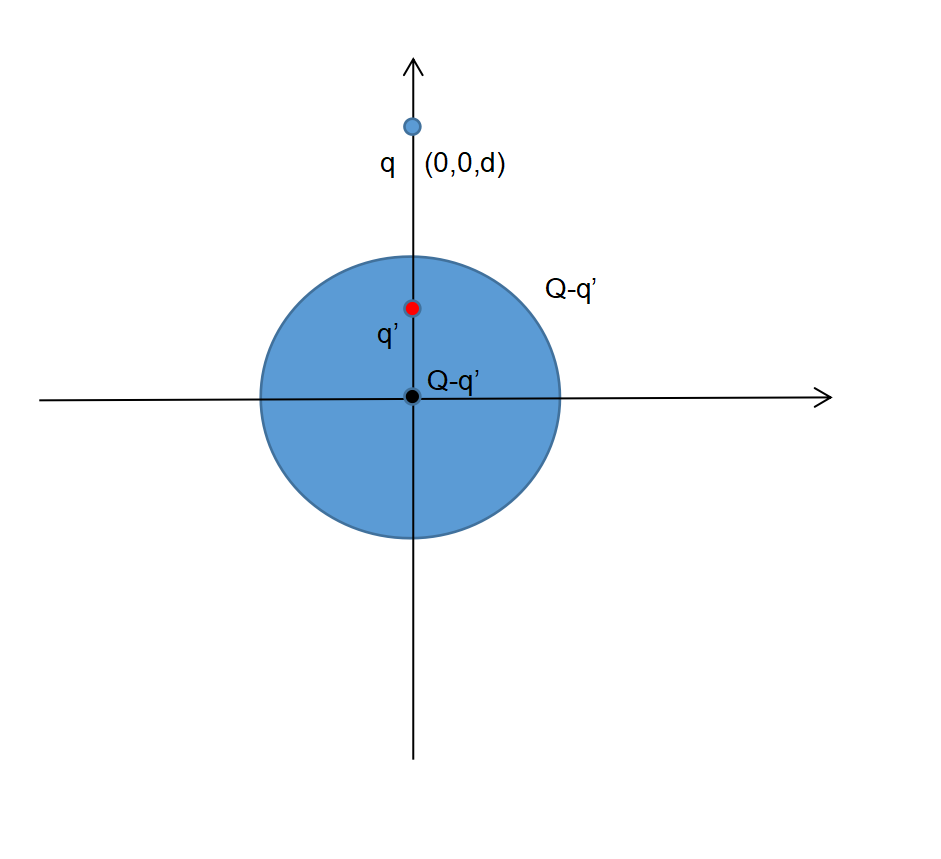
\includegraphics[width=0.5\textwidth]{fig1.png}\caption{Image charge}
      \label{fig1}
    \end{figure}

    The image charge $q'$ is shown in Figure~\ref{fig1}. Then, the outer surface will induce a charge distribution of $Q-q'$, which can be viewed as a point charge at the origin. Hence the electric potential distribution outside the sphere is:
    \begin{equation}
      q:(0,0,d),\quad \quad q'=-\dfrac{a}{d}q:(0,0,\dfrac{a^2}{d}),\quad \quad Q-q'=Q+\dfrac{a}{d}q:(0,0,0) \nonumber
    \end{equation}
    \begin{eqnarray}
      \phi(\boldsymbol{r})=\phi(r,\theta)=\dfrac{1}{4\pi\epsilon_0}\left[\dfrac{q}{\sqrt{r^2+d^2-2rd\cos\theta}}-\dfrac{\dfrac{a}{d}q}{\sqrt{\dfrac{a^4}{d^2}+r^2-2\dfrac{a^2}{d}r\cos\theta}}+\dfrac{Q+\dfrac{a}{d}q}{r}\right]
    \end{eqnarray}

    \item Calculate the electric field distribution outside the sphere.
    \begin{eqnarray}
      \boldsymbol{E}=-\nabla\phi&=&-\dfrac{1}{4\pi\epsilon_0}\left[\dfrac{(d\cos\theta-r)q}{(r^2+d^2-2rd\cos\theta)^{\frac{3}{2}}}-\dfrac{(\dfrac{a^2}{d}\cos\theta-r)\dfrac{a}{d}q}{{(r^2+\dfrac{a^4}{d^2}-2r\dfrac{a^2}{d}\cos\theta)}^{\frac{3}{2}}}-\dfrac{Q+\dfrac{a}{d}q}{r^2}\right]\hat{r}\nonumber \\
      &&-\dfrac{1}{4\pi\epsilon_0}\left[\dfrac{-qd\sin\theta}{{(r^2+d^2-2rd\cos\theta)}^{\frac{3}{2}}}+\dfrac{q\dfrac{a^3}{d^2}\sin\theta}{{(r^2+\dfrac{a^4}{d^2}-2r\dfrac{a^2}{d}\cos\theta)}^{\frac{3}{2}}}\right]\hat{\theta}
    \end{eqnarray}

    \item Calculate the surface charge density distribution $\sigma$ at the conducting sphere, and calculate the Coulomb force per unit area exerted on the surface charge.
    \begin{eqnarray}
      \sigma&=&-\epsilon_0\left.\dfrac{\partial\phi}{\partial r}\right|_{r=a}\nonumber \\
      &=&-\dfrac{1}{4\pi}\left[\dfrac{(d\cos\theta-a)q}{{(a^2+d^2-2ad\cos\theta)}^{\frac{3}{2}}}-\dfrac{(\dfrac{a^2}{d}\cos\theta-a)\dfrac{a}{d}q}{{(a^2+\dfrac{a^4}{d^2}-2a\dfrac{a^2}{d}\cos\theta)}^{\frac{3}{2}}}-\dfrac{Q+\dfrac{a}{d}q}{a^2}\right]\nonumber \\
      &=&-\dfrac{q}{4\pi a^2}\dfrac{a}{d}\left[\dfrac{1-\dfrac{a^2}{d^2}}{{(1+\dfrac{a^2}{d^2}-2\dfrac{a}{d}\cos\theta)}^{\frac{3}{2}}}-\dfrac{d}{a}\dfrac{Q}{q}-1\right]
    \end{eqnarray}

    The force per unit area is $dF=\dfrac{\sigma^2}{2\epsilon_0}dS$
    \begin{equation}
      dF=\dfrac{q^2}{32\pi^2a^2d^2\epsilon_0}\left[\dfrac{1-\dfrac{a^2}{d^2}}{{(1+\dfrac{a^2}{d^2}-2\dfrac{a}{d}\cos\theta)}^{\frac{3}{2}}}-\dfrac{d}{a}\dfrac{Q}{q}-1\right]^2
    \end{equation}

    \item Calculate the surface Coulomb force $F$ exerted on the point charge $q$ from the charged sphere. Let charge $q=1,Q=6q,a=1$, numerically calculate this force, and plot $F$ as a function of $d$.
    
    Using method of the image, the force on the point charge $q$ is:
    \begin{equation}
      F = \dfrac{1}{4\pi\epsilon_0}\left[\dfrac{q(Q+\frac{a}{d}q)}{d^2}-\dfrac{q(\frac{a}{d}q)}{(d-\frac{a^2}{d})^2}\right]
    \end{equation}
    With the numerical settings:
    \begin{equation}
      F = \dfrac{1}{4\pi\epsilon_0}\left[\dfrac{6}{d^2}+\dfrac{1}{d^3}-\dfrac{d}{(d^2-1)^2}\right]
    \end{equation}
    \begin{figure}[h]
      \centering
      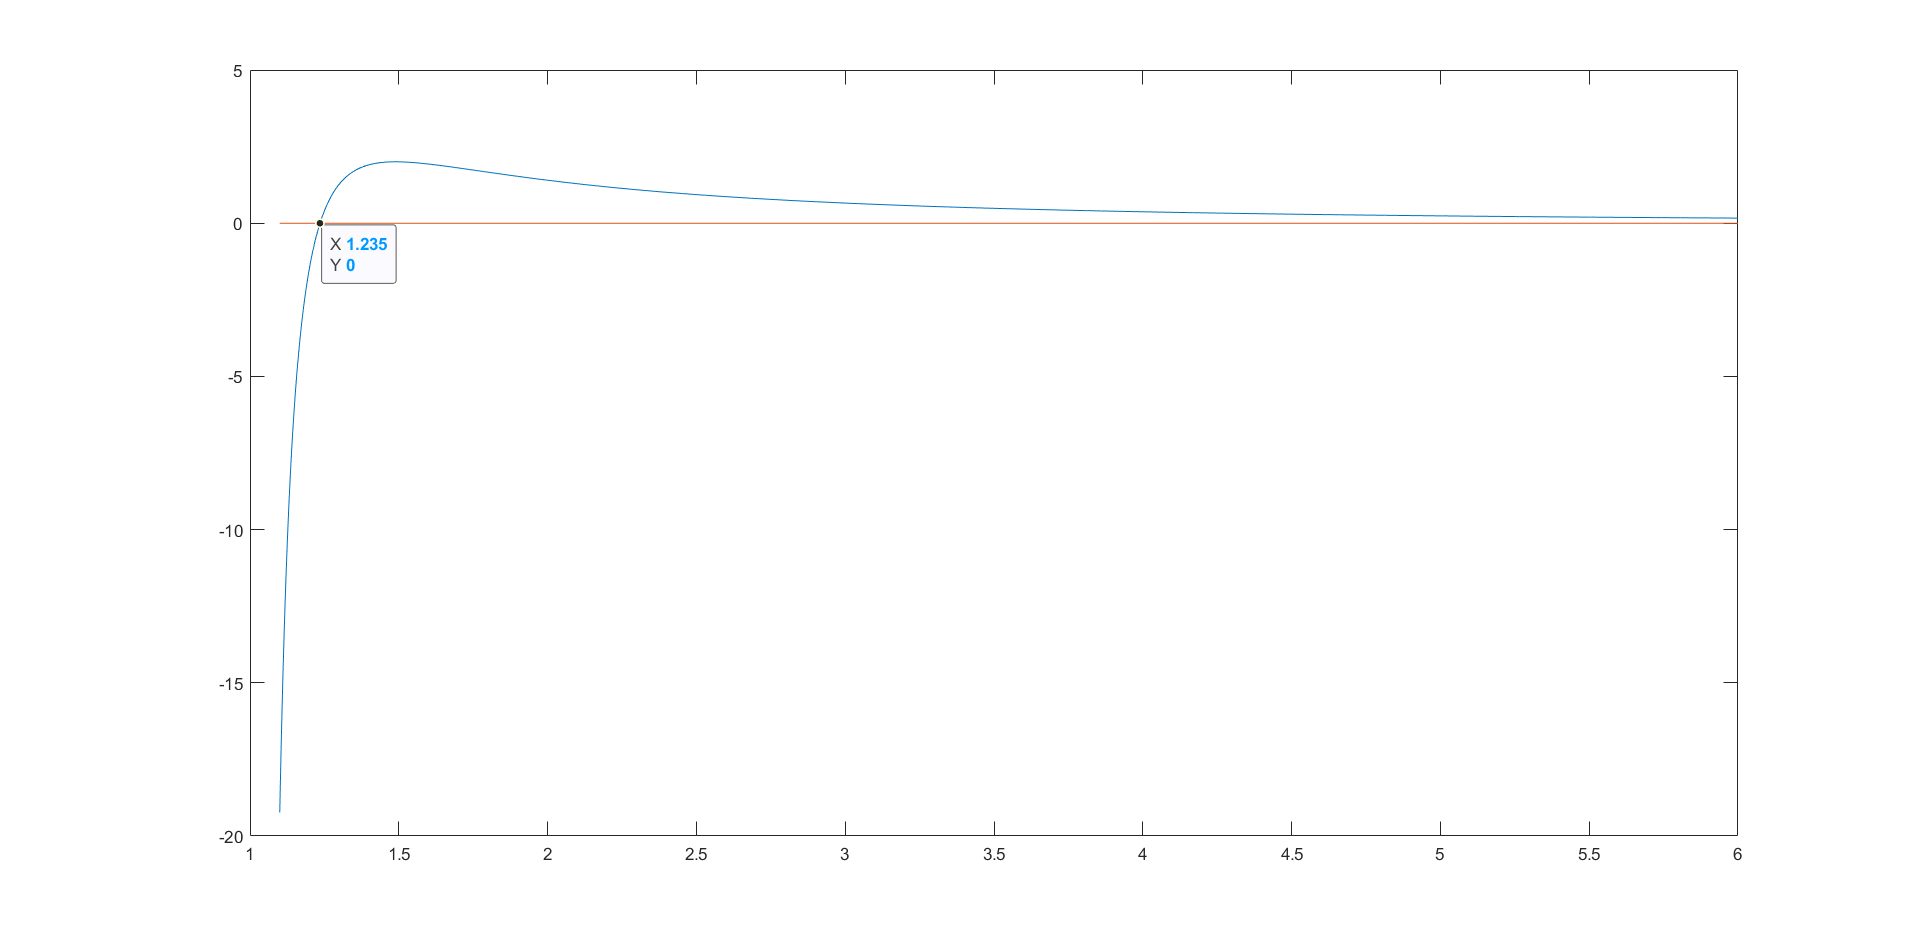
\includegraphics[width=0.7\textwidth]{fig4.png}\caption{the \textit{force} of $d$}
    \end{figure}
    Here, the sign $``+"$ represents repulsive.

    \item Consider the limit of $Q\gg q$, is the Coulomb force always repulsive? At which point $d=d_c$, the force becomes attractive? Derive an analytic expression for $d_c$(in the limit of $Q\gg q$) to the leading order of $\dfrac{q}{Q}$. Compare this analytic expression with the numerical value of $d_c$ for $Q=6q$ obtained in $(d)$.
    
    No, when $d$ is small enough, the force will become attractive. Set $q/Q = x$, then the force is:
    \begin{eqnarray}
      F
      &=&\dfrac{1}{4\pi\epsilon_0}\left[\dfrac{xQ^2+\frac{a}{d}x^2Q^2}{d^2}-\dfrac{q^2\frac{a}{d}}{(d-\frac{a^2}{d})^2}\right]\nonumber\\
      &\approx& \dfrac{1}{4\pi\epsilon_0}\left[\dfrac{xQ^2}{d^2}-\dfrac{q^2\frac{a}{d}}{(d-\frac{a^2}{d})^2}\right]
    \end{eqnarray}
    Set $F=0$, the equation is:
    \begin{eqnarray}
      adx=(d-\dfrac{a^2}{d})^2 \nonumber \\
      d_c^4-axd_c^3-2a^2d_c^2+a^4=0
    \end{eqnarray}

    Let $a=1,x=\frac{1}{6}$, we can numerically solve the equation:
    \begin{figure}[h]
      \centering
      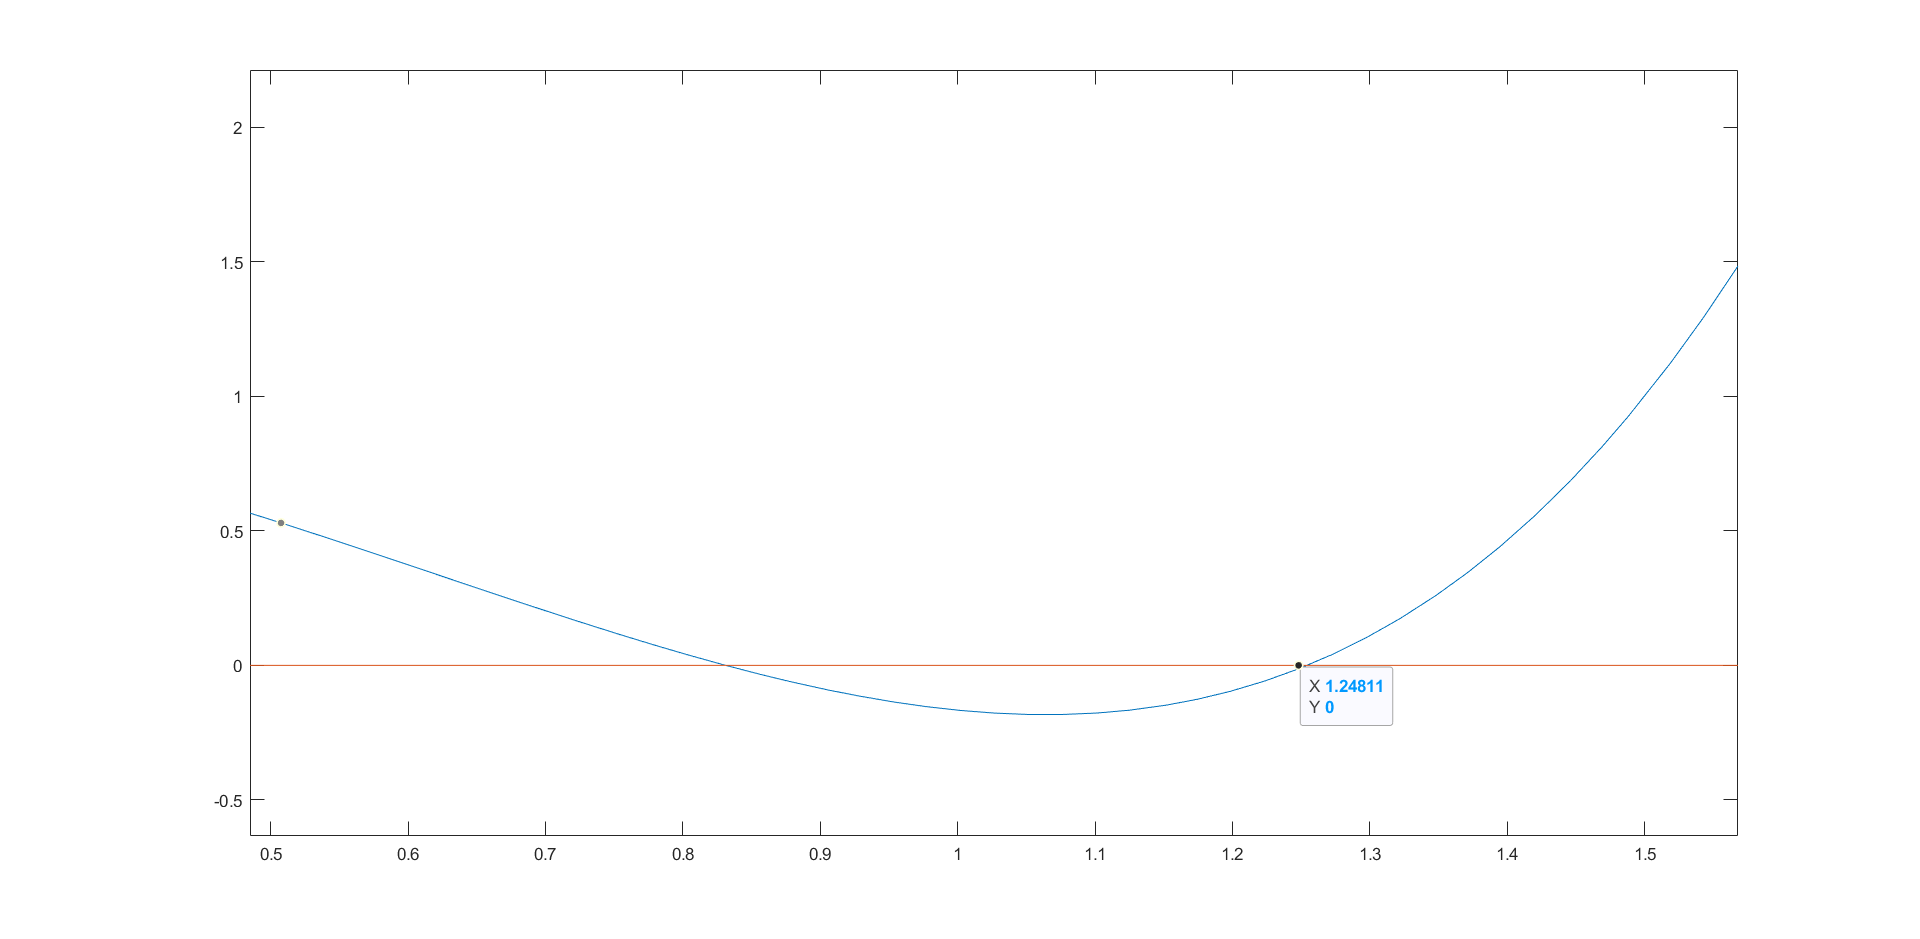
\includegraphics[width=0.8\textwidth]{fig5.png}\caption{numerical solution}
    \end{figure}
  \end{enumerate}

  \item A point charge $q$ is brought to a position a distribution $d$ away from an infinite plane condutor held at zero potential. Using the method of images, find:
  \begin{enumerate}
    \item the surface-charge density $\sigma$ induced on the plane, and plot it:
    \begin{figure}[h]
      \centering
      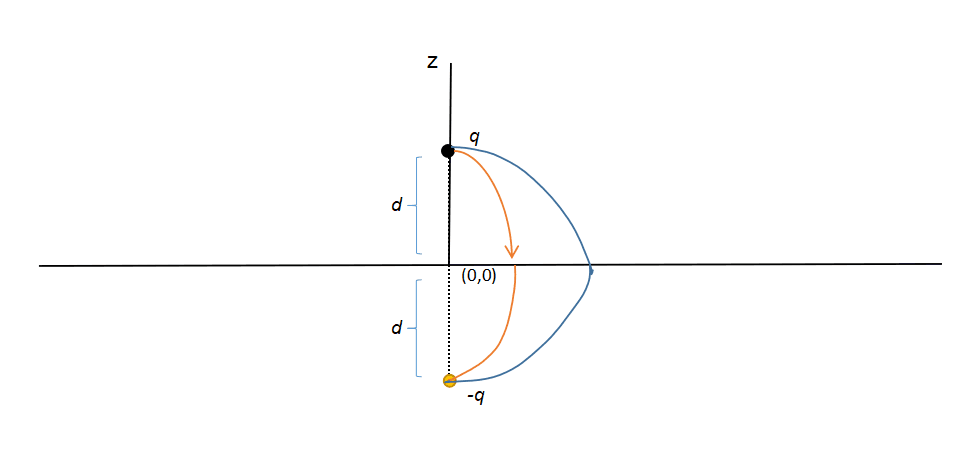
\includegraphics[width=0.8\textwidth]{fig2.png}\caption{charge potential distribution}
      \label{fig2}
    \end{figure}

    The illustration is shown in Figure~\ref{fig2}, and by the symmetry, we use $\phi(\rho,z)$ to describe the potential. Since the on the plane, the potential is zero, hence the potential distribution is:
    \begin{equation}
      \phi(\rho,z)=\dfrac{q}{4\pi\epsilon_0}\left[\dfrac{1}{\sqrt{{(d-z)}^2+\rho^2}}-\dfrac{1}{\sqrt{{(d+z)}^2+\rho^2}}\right]
    \end{equation}

    Then the surface charge density is:
    \begin{eqnarray}
      \sigma=-\epsilon_0\left.\dfrac{\partial\phi}{\partial z}\right|_{z=0}
      &=&-\dfrac{q}{4\pi}\left.\left[\dfrac{d-z}{{({(d-z)}^2+\rho^2)}^{\frac{3}{2}}}-\dfrac{d+z}{{({(d+z)}^2+\rho^2)}^{\frac{3}{2}}}\right]\right|_{z=0}\nonumber \\
      &=&-\dfrac{qd}{2\pi{(d^2+\rho^2)}^{\frac{3}{2}}}
    \end{eqnarray}
    \begin{figure}[h]
      \centering
      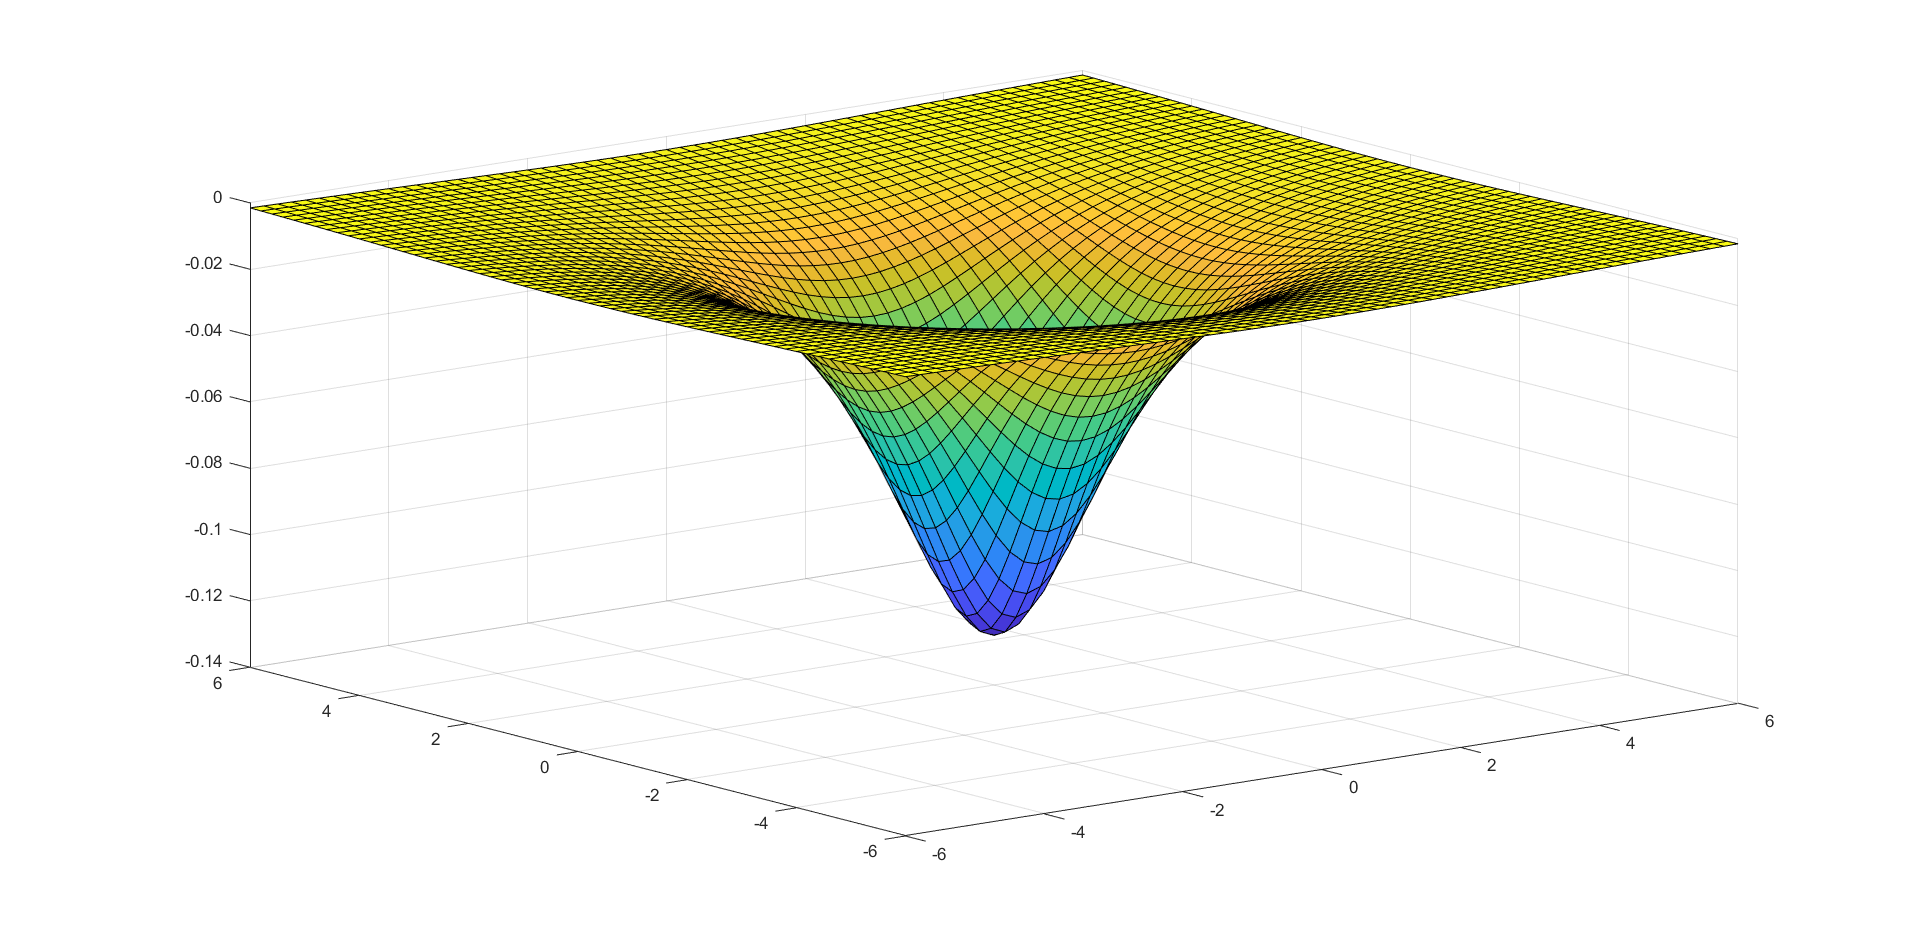
\includegraphics[width=1\textwidth]{fig3.png}\caption{surface charge density distribution}
    \end{figure}
    \item the force between the plane and the charge by using Coulomb's law for the force between the charge and its image:
    \begin{equation}
      |F|=\frac{1}{4\pi\epsilon_0}\dfrac{q^2}{(2d)^2}=\dfrac{q^2}{16\pi\epsilon_0 d^2} 
    \end{equation}

    \item the total force acting on the plane by integrating $\dfrac{\sigma^2}{2\epsilon_0}$ over the whole plane:
    \begin{eqnarray}
      |F|&=&\int^{2\pi}_0 d\theta \int^{\infty}_0 \rho d\rho \dfrac{\sigma^2}{2\epsilon_0}\nonumber \\
      &=&\dfrac{q^2}{4\pi\epsilon_0}\int^{\infty}_0d\rho \dfrac{d^2\rho}{{(d^2+\rho^2)}^3}\\
      &=&\dfrac{q^2}{4\pi\epsilon_0 d^2}\int^{\infty}_0dx\dfrac{x}{{(1+x^2)}^3}\\
      &=&\left.\dfrac{q^2}{4\pi\epsilon_0 d^2}\dfrac{1}{2}(-\dfrac{1}{2})\dfrac{1}{{(1+x^2)}^2}\right|^{\infty}_0\\
      &=&\dfrac{q^2}{16\pi\epsilon_0 d^2} 
    \end{eqnarray}

    \item the work necessary to remove the charge $q$ from its position to infinity:
    \begin{eqnarray}
      W = q\times(\phi(z=\infty,\rho=0)-\phi(z=d,\rho=0))=\dfrac{q^2}{8\pi\epsilon_0d}
    \end{eqnarray}
  \end{enumerate}

  \item About the Legendre functions $\{P_l(x)\}$
  \begin{enumerate}
    \item Derive Rodrigues'formula:$\quad\quad P_l(x)=\dfrac{1}{2^l l!}\dfrac{d^l}{dx^l}{(x^2-1)}^l$
    
    The general Legendre functions is:
    \begin{equation}
      P_l(x)=\sum\limits^{\lceil\frac{l-1}{2}\rceil}_{k=0}{(-1)}^k\dfrac{(2l-2k)!}{2^l k!(l-k)!(l-2k)!}x^{l-2k}
    \end{equation} 

    Using the binomial therorem:
    \begin{eqnarray}
      \dfrac{1}{2^l l!}\dfrac{d^l}{dx^l}{(x^2-1)}^l
      &=&\dfrac{1}{2^l l!}\dfrac{d^l}{dx^l}\sum\limits_{k=0}^{l}C^{k}_{l}{(-1)}^{k}x^{2l-2k}\nonumber \\
      &=&\dfrac{1}{2^l l!}\sum\limits_{k=0}^{\lceil\frac{l-1}{2}\rceil}C^{k}_{l}{(-1)}^{k}(2l-2k)(2l-2k-1)\dotsm(l-2k+1)x^{l-2k}\nonumber \\
      &=&\sum\limits_{k=0}^{\lceil\frac{l-1}{2}\rceil}{(-1)}^{k}\dfrac{l!(2l-2k)!}{2^l l!k!(l-k)!(l-2k)!}x^{l-2k}\nonumber \\
      &=&\sum\limits^{\lceil\frac{l-1}{2}\rceil}_{k=0}{(-1)}^k\dfrac{(2l-2k)!}{2^l k!(l-k)!(l-2k)!}x^{l-2k}=P_l(x)
    \end{eqnarray}

    \item Derive $\quad \dfrac{dP_{l+1}}{dx}-\dfrac{dP_{l-1}}{dx}-(2l+1)P_l=0$
    
    Proof:
    \begin{eqnarray}
      \dfrac{dP_{l+1}}{dx}
      &=&\dfrac{d}{dx}\sum\limits^{\lceil\frac{l}{2}\rceil}_{k=0}{(-1)}^k\dfrac{(2l+2-2k)!}{2^{l+1} k!(l+1-k)!(l+1-2k)!}x^{l+1-2k}\nonumber \\
      &=&\sum\limits^{\lceil\frac{l}{2}\rceil}_{k=0}{(-1)}^k\dfrac{(2l+2-2k)!}{2^{l+1} k!(l+1-k)!(l-2k)!}x^{l-2k}
    \end{eqnarray}
    \begin{eqnarray}
      \dfrac{dP_{l-1}}{dx}
      &=&\dfrac{d}{dx}\sum\limits^{\lceil\frac{l-2}{2}\rceil}_{k=0}{(-1)}^k\dfrac{(2l-2-2k)!}{2^{l-1} k!(l-1-k)!(l-1-2k)!}x^{l-1-2k}\nonumber \\
      &=&\sum\limits^{\lceil\frac{l-2}{2}\rceil}_{k=0}{(-1)}^k\dfrac{(2l-2-2k)!}{2^{l-1} k!(l-1-k)!(l-2-2k)!}x^{l-2-2k}
    \end{eqnarray}
      
    \begin{eqnarray}
      \dfrac{dP_{l+1}}{dx}-\dfrac{dP_{l-1}}{dx}&=&\dfrac{(2l+2)!}{2^{l+1}(l+1)!l!}x^{l}+\sum\limits_{k=1}^{\lceil\frac{l}{2}\rceil}\Big[{(-1)}^k\dfrac{(2l+2-2k)!}{2^{l+1}k!(l+1-k)!(l-2k)!}\nonumber \\
      &&-{(-1)}^{k-1}\dfrac{(2l-2k)!}{2^{l-1} (k-1)!(l-k)!(l-2k)!}\Big]x^{l-2k}\nonumber \\
      &=& (2l+1)\dfrac{(2l)!}{2^l l!l!}x^l+\sum\limits_{k=1}^{\lceil\frac{l}{2}\rceil}\Big[{(-1)}^k\dfrac{(2l-2k)!}{2^{l}k!(l-k)!(l-2k)!}\nonumber \\
      &&(\dfrac{(2l+2-2k)(2l+1-2k)}{2(l+1-k)}+2k)\Big]x^{l-2k}\nonumber \\
      &=&(2l+1)\sum\limits^{\lceil\frac{l-1}{2}\rceil}_{k=0}{(-1)}^k\dfrac{(2l-2k)!}{2^l k!(l-k)!(l-2k)!}x^{l-2k}\nonumber \\
      &=&(2l+1)P_l
    \end{eqnarray}
    
    Hence,$\quad \dfrac{dP_{l+1}}{dx}-\dfrac{dP_{l-1}}{dx}-(2l+1)P_l=0$
    
    \item Using the identity $(l+1)P_{l+1}-(2l+1)xP_l+lP_{l-1}=0$ to calculate the following integral:
    \begin{equation}
      I_2=\int^{1}_{-1}dx x^2 P_l(x)P_{l'}(x) \nonumber
    \end{equation}
    
    \begin{eqnarray}
      I_2
      &=&\int^{1}_{-1}dx(xP_l)(xP_{l'})\nonumber \\
      &=&\int^{1}_{-1}dx(\dfrac{(l+1)P_{l+1}+lP_{l-1}}{2l+1})(\dfrac{(l'+1)P_{l'+1}+l'P_{l'-1}}{2l'+1})\nonumber \\
      &=&\int^{1}_{-1}dx\dfrac{(l+1)(l'+1)}{(2l+1)(2l'+1)}P_{l+1}P_{l'+1}+\dfrac{l(l'+1)}{(2l+1)(2l'+1)}P_{l-1}P_{l'+1}+\dotso\nonumber \\
      &=&\dfrac{2{(l+1)}^2}{{(2l+1)}^2(2l+3)}\delta_{l,l'}+\dfrac{2l(l-1)}{(2l+1)(2l-1)(2l-3)}\delta_{l-1,l'+1}+\dotso\nonumber \\
      &=&\begin{cases}
        \dfrac{2{(l+1)}^2}{{(2l+1)}^2(2l+3)}+\dfrac{2l^2}{{(2l+1)}^2(2l-1)}\quad\quad\quad\quad\quad l=l' \\
        \dfrac{2l(l-1)}{(2l+1)(2l-1)(2l-3)}\quad\quad\quad\quad\quad\quad\quad\quad\quad\quad l=l'+2 \\
        \dfrac{2(l+1)(l+2)}{(2l+1)(2l+3)(2l+5)}\quad\quad\quad\quad\quad\quad\quad\quad\quad\quad l=l'-2
      \end{cases}
    \end{eqnarray}
  \end{enumerate}

  \item Numerically solve Poisson equation in two dimension:
  \begin{equation}\label{eq:poisson}
    \dfrac{\partial^2\phi(x,y)}{\partial x^2}+\dfrac{\partial^2\phi(x,y)}{\partial y^2}=-\dfrac{\rho(x,y)}{\epsilon_0}
  \end{equation}

  Solve the potential inside the rectangle of length $L$ and width $W$. The rectangle is divided into $N_x\times N_y$ discrete sites$(L=2W=2m)$:
  \begin{eqnarray}
    r_{i,j}=(x_i,y_j)=(\dfrac{iL}{N_x},\dfrac{jW}{N_y})=(ih_x,jh_y) \quad\quad\quad\quad 0 \leqslant i \leqslant N_x, 0 \leqslant j \leqslant N_y
  \end{eqnarray}
  with boundary condition $\phi_0=1V$:
  \begin{eqnarray}
    \phi(x=0,y)=0,\phi(x=L,y)=\phi_0 \quad\quad\quad \phi(x,y=0)=\dfrac{\phi_0 x}{L},\phi(x,y=W)=\dfrac{\phi_0 x}{L}
  \end{eqnarray}
  Then the Poisson equation in matrix form:
  \begin{equation}
    \boldsymbol{A}\cdot\boldsymbol{\phi}=-\dfrac{\boldsymbol{\rho}}{\epsilon_0}+\boldsymbol{b}
  \end{equation}

  \begin{enumerate}
    \item Charge density is zero inside the rectangle,$\quad\rho(\boldsymbol{r})=0$
    
    The second difference equation is:
    \begin{eqnarray}
      \begin{cases}
        \left.\dfrac{\partial^2\phi}{\partial x^2}\right|_{x=x_i,y=y_j}=\dfrac{\phi_{i+1,j}-2\phi_{i,j}+\phi_{i-1,j}}{h_x^{2}} \\
        \left.\dfrac{\partial^2\phi}{\partial y^2}\right|_{x=x_i,y=y_j}=\dfrac{\phi_{i,j+1}-2\phi_{i,j}+\phi_{i,j-1}}{h_y^{2}}
      \end{cases}
    \end{eqnarray}

    Then we can translate the Eq~(\ref{eq:poisson}) into the linear equations:
    \begin{eqnarray}
      \begin{cases}
        \dfrac{1}{h_x^2}\phi_{i+1,j}+\dfrac{1}{h_y^2}\phi_{i,j+1}-2(\dfrac{1}{h_x^2}+\dfrac{1}{h_y^2})\phi_{i,j}+\dfrac{1}{h_x^2}\phi_{i-1,j}+\dfrac{1}{h_y^2}\phi_{i,j-1}=b_{i,j}\\
        \phi_{0,j}=0,\phi_{N_x,j}=\phi_0,\phi_{i,0}=\dfrac{i}{N_x}\phi_0,\phi_{i,N_y}=\dfrac{i}{N_x}\phi_0
      \end{cases}
    \end{eqnarray}

    Reset the vector:
    \begin{equation}
      \phi_{j}^{h}=
        \begin{array}{|c|}
          \phi_{1,j}\\
          \phi_{2,j}\\
          \vdots\\
          \phi_{N_x-1,j}
        \end{array}
      \quad
      b_{j}^{h}=
        \begin{array}{|c|}
          b_{1,j}\\
          b_{2,j}\\
          \vdots\\
          b_{N_x-1,j}
        \end{array}
      \quad
      \phi^{h}=
        \begin{array}{|c|}
          \phi^{h}_{1}\\
          \phi^{h}_{2}\\
          \vdots\\
          \phi^{h}_{N_y-1}
        \end{array}
      \quad
      b^{h}=
        \begin{array}{|c|}
          b^{h}_{1}\\
          b^{h}_{2}\\
          \vdots\\
          b^{h}_{N_y-1}
        \end{array}
      \nonumber
    \end{equation}
    \begin{equation}    
      C=
          \begin{bmatrix}
            -2(\frac{1}{h_x^2}+\frac{1}{h_y^2})&\frac{1}{h_x^2}&\cdots \\
            \frac{1}{h_x^2} & -2(\frac{1}{h_x^2}+\frac{1}{h_y^2}) & \frac{1}{h_x^2} \\
            &\ddots & \ddots & \ddots \\
            &  & \frac{1}{h_x^2}&-2(\frac{1}{h_x^2}+\frac{1}{h_y^2}) & \frac{1}{h_x^2} \\
            &  &  & \frac{1}{h_x^2}&-2(\frac{1}{h_x^2}+\frac{1}{h_y^2})
          \end{bmatrix}_{(N_x-1)\times (N_x-1)}
    \end{equation}
    \begin{equation}
      A=
          \begin{bmatrix}
              C & \frac{1}{h_y^2}I & \cdots \\
              \frac{1}{h_y^2}I & C & \frac{1}{h_y^2}I \\
              &\ddots & \ddots & \ddots \\
              &  & \frac{1}{h_y^2}I & C & \frac{1}{h_y^2}I \\
              &  &   & \frac{1}{h_y^2}I & C
          \end{bmatrix}    
    \end{equation}
    Hence the equation can be written as:
    \begin{eqnarray}
      A\phi^{h}=b^{h}
    \end{eqnarray}
    with $b^{h}$
    \begin{equation}
      -b_{1}^{h}=
        \begin{array}{|c|}
          \frac{1}{h_y^2N_x}\phi_0\\
          \frac{2}{h_y^2N_x}\phi_0\\
          \vdots\\
          (\frac{N_x-1}{h_y^2N_x}+\frac{1}{h_x^2})\phi_0
        \end{array}
      \quad
      -b_{N_y-1}^{h}=
        \begin{array}{|c|}
          \frac{1}{h_y^2N_x}\phi_0\\
          \frac{2}{h_y^2N_x}\phi_0\\
          \vdots\\
          (\frac{N_x-1}{h_y^2N_x}+\frac{1}{h_x^2})\phi_0
        \end{array}
      \nonumber
      \quad
      \begin{cases}
        -b_{N_x-1,j}=\frac{1}{h_x^2}\phi_0\quad(j\neq 1,N_y-1)\\
        -b_{i,j}=0\quad(i\neq 1,N_x-1;j\neq 1,N_y-1)
      \end{cases}
    \end{equation}

    The potential distribution is:
    \begin{figure}[h]
      \centering
      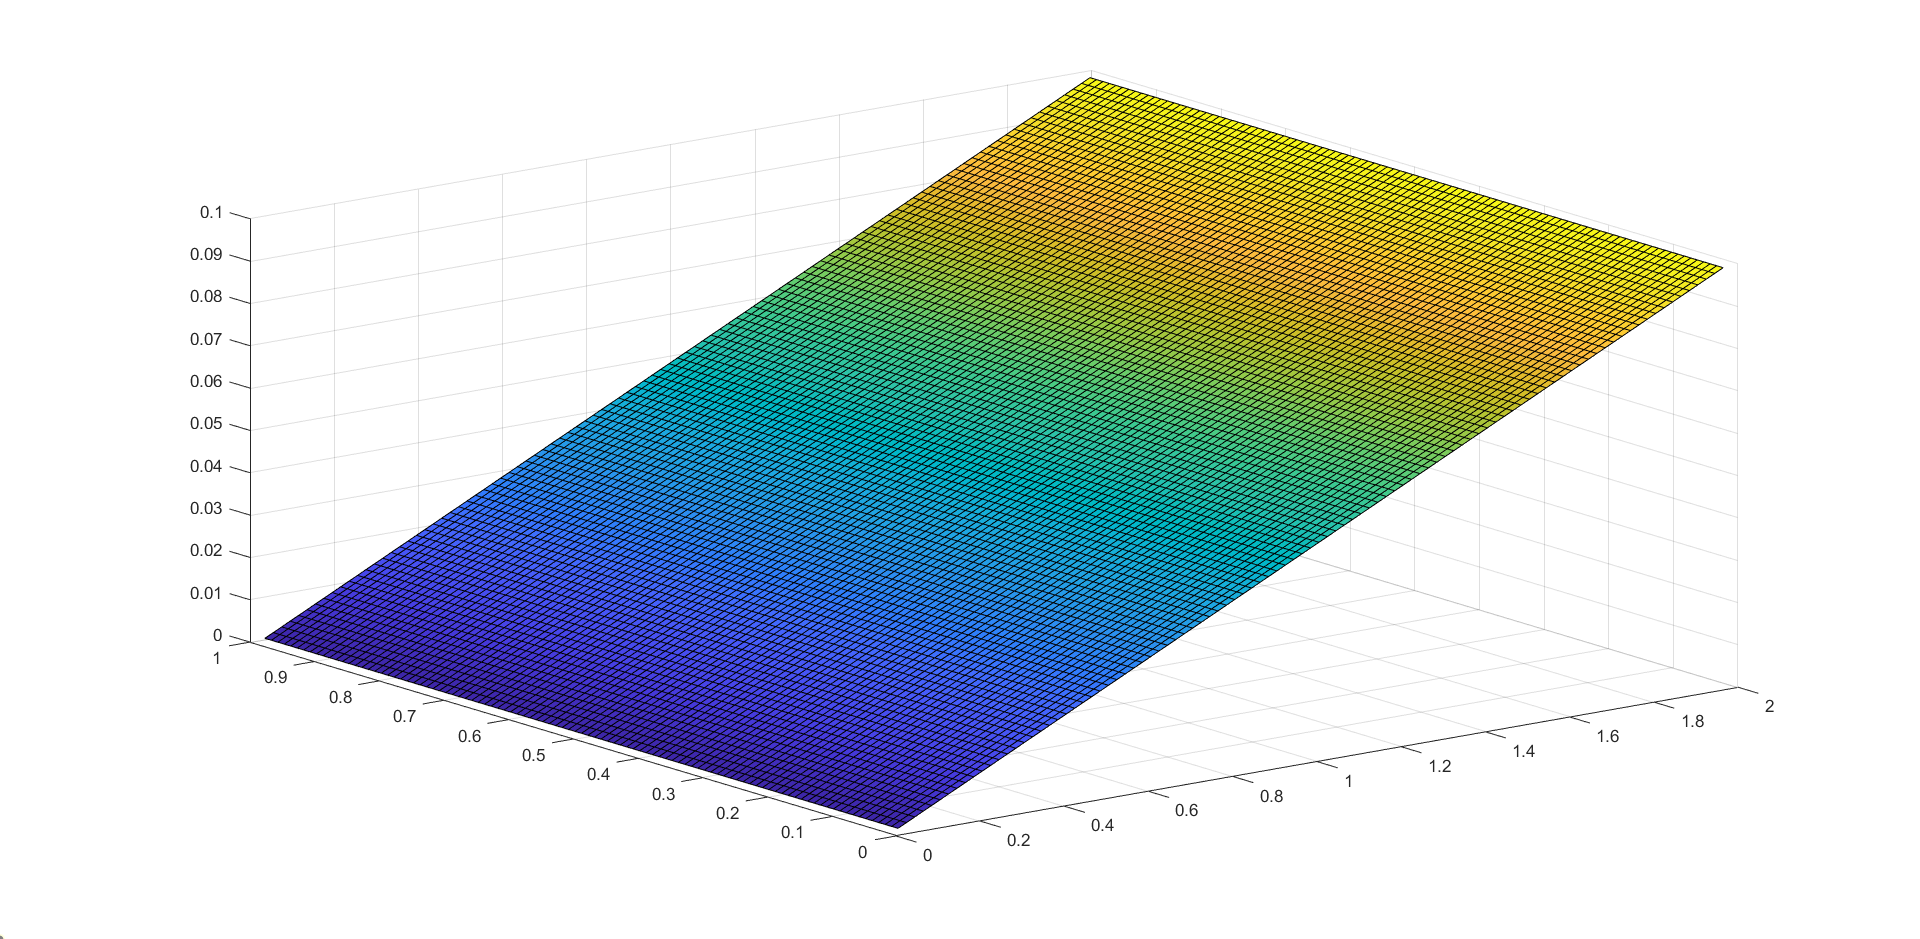
\includegraphics[width=0.75\textwidth]{fig6.png}\caption{The electrostatic potentials for $\rho(\boldsymbol{r})=0$}
    \end{figure}
    
    \item Charge density obeys a Gaussian distribution,$\quad\rho(\boldsymbol{r})=\rho_0e^{-20\frac{|\boldsymbol{r}-\boldsymbol{r}_c|^2}{W^2}},\boldsymbol{r}_c=(\frac{L}{2},\frac{W}{2}),\rho_0=1\quad C/m^2$  
    
    The equation becomes:
    \begin{equation}
      A\phi^{h}=b^{h}-\dfrac{\rho^{h}}{\epsilon_0}
    \end{equation}

    After numerical calculation, the potential distribution is as the following:
    \begin{figure}[h]
      \centering
      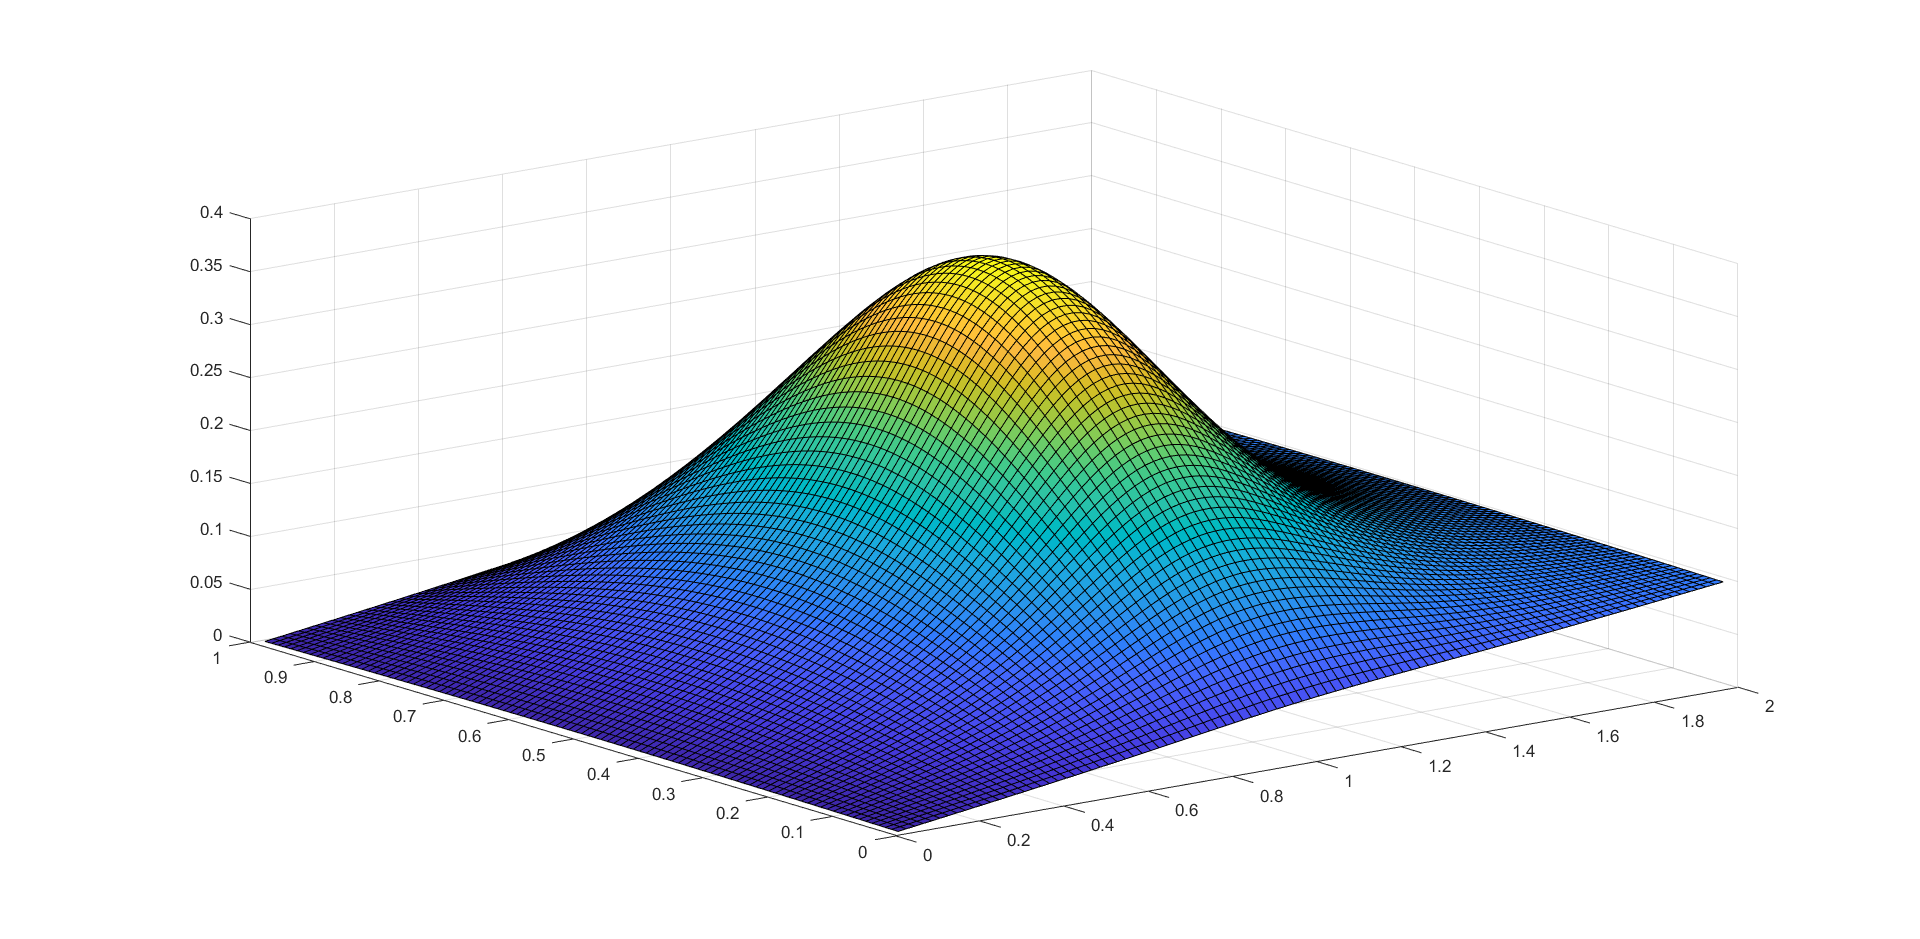
\includegraphics[width=0.75\textwidth]{fig7.png}\caption{The electrostatic potential for $\rho(\boldsymbol{r})=\rho_0e^{-20|\boldsymbol{r}-\boldsymbol{r}_c|^2/W^2}$}
    \end{figure}
  \end{enumerate}
\end{enumerate}


Here is my code:
\lstinputlisting{poisson.m}

\end{document}